% Generated by ArticleSignalDiagrams. Opaque vector fills only.
\documentclass[10pt,tikz,border=5pt]{standalone}
\usepackage{lmodern}
\usetikzlibrary{fit}
\begin{document}
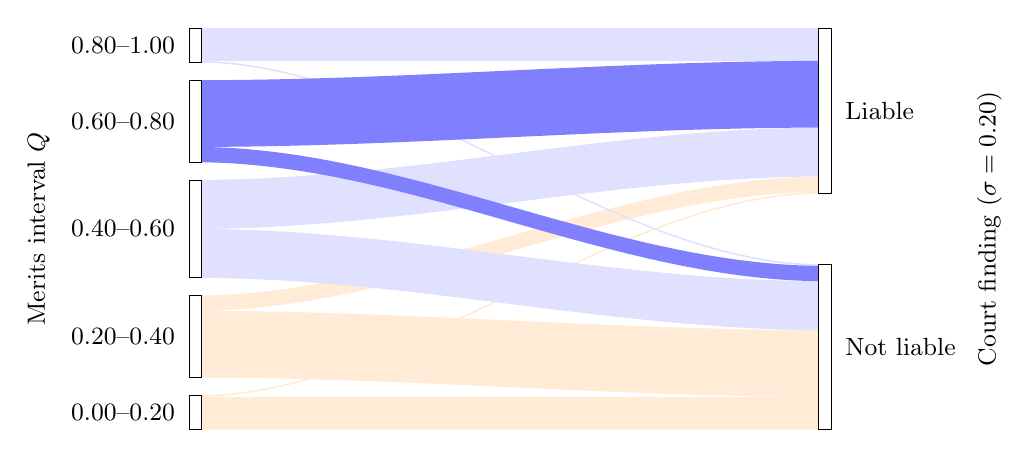
\begin{tikzpicture}[x=1cm,y=1cm,font=\small]\path[fill=orange!16!white,draw=none] (3.3,-5.1) .. controls (6,-5.1) and (8.6,-5.1) .. (11.3,-5.1) -- (11.3,-4.683738) .. controls (8.6,-4.683738) and (6,-4.683738) .. (3.3,-4.683738) -- cycle;
\path[fill=orange!16!white,draw=none] (3.3,-4.683738) .. controls (6,-4.683738) and (8.6,-2.1) .. (11.3,-2.1) -- (11.3,-2.079462) .. controls (8.6,-2.079462) and (6,-4.6632) .. (3.3,-4.6632) -- cycle;
\path[fill=orange!16!white,draw=none] (3.3,-4.4382) .. controls (6,-4.4382) and (8.6,-4.683738) .. (11.3,-4.683738) -- (11.3,-3.836414) .. controls (8.6,-3.836414) and (6,-3.590876) .. (3.3,-3.590876) -- cycle;
\path[fill=orange!16!white,draw=none] (3.3,-3.590876) .. controls (6,-3.590876) and (8.6,-2.079462) .. (11.3,-2.079462) -- (11.3,-1.885186) .. controls (8.6,-1.885186) and (6,-3.3966) .. (3.3,-3.3966) -- cycle;
\path[fill=blue!12!white,draw=none] (3.3,-3.1716) .. controls (6,-3.1716) and (8.6,-3.836414) .. (11.3,-3.836414) -- (11.3,-3.214814) .. controls (8.6,-3.214814) and (6,-2.55) .. (3.3,-2.55) -- cycle;
\path[fill=blue!12!white,draw=none] (3.3,-2.55) .. controls (6,-2.55) and (8.6,-1.885186) .. (11.3,-1.885186) -- (11.3,-1.263586) .. controls (8.6,-1.263586) and (6,-1.9284) .. (3.3,-1.9284) -- cycle;
\path[fill=blue!12!white,draw=none] (3.3,-0.4368) .. controls (6,-0.4368) and (8.6,-3.020538) .. (11.3,-3.020538) -- (11.3,-3) .. controls (8.6,-3) and (6,-0.416262) .. (3.3,-0.416262) -- cycle;
\path[fill=blue!12!white,draw=none] (3.3,-0.416262) .. controls (6,-0.416262) and (8.6,-0.416262) .. (11.3,-0.416262) -- (11.3,0) .. controls (8.6,0) and (6,0) .. (3.3,0) -- cycle;
\path[fill=blue!50!white,draw=none] (3.3,-1.7034) .. controls (6,-1.7034) and (8.6,-3.214814) .. (11.3,-3.214814) -- (11.3,-3.020538) .. controls (8.6,-3.020538) and (6,-1.509124) .. (3.3,-1.509124) -- cycle;
\path[fill=blue!50!white,draw=none] (3.3,-1.509124) .. controls (6,-1.509124) and (8.6,-1.263586) .. (11.3,-1.263586) -- (11.3,-0.416262) .. controls (8.6,-0.416262) and (6,-0.6618) .. (3.3,-0.6618) -- cycle;
\coordinate (axis-midline-0) at (0,-2.55);
\path[fill=white,draw=black,line width=0.3pt] (3.22,-5.1) rectangle (3.38,-4.6632);
\node[anchor=east,fill=white,inner sep=2pt] (bucket-0-0-0) at (3.12,-4.8816) {0.00--0.20};
\path[fill=white,draw=black,line width=0.3pt] (3.22,-4.4382) rectangle (3.38,-3.3966);
\node[anchor=east,fill=white,inner sep=2pt] (bucket-0-0-1) at (3.12,-3.9174) {0.20--0.40};
\path[fill=white,draw=black,line width=0.3pt] (3.22,-3.1716) rectangle (3.38,-1.9284);
\node[anchor=east,fill=white,inner sep=2pt] (bucket-0-0-2) at (3.12,-2.55) {0.40--0.60};
\path[fill=white,draw=black,line width=0.3pt] (3.22,-1.7034) rectangle (3.38,-0.6618);
\node[anchor=east,fill=white,inner sep=2pt] (bucket-0-0-3) at (3.12,-1.1826) {0.60--0.80};
\path[fill=white,draw=black,line width=0.3pt] (3.22,-0.4368) rectangle (3.38,0);
\node[anchor=east,fill=white,inner sep=2pt] (bucket-0-0-4) at (3.12,-0.2184) {0.80--1.00};
\node[fit=(bucket-0-0-0) (bucket-0-0-1) (bucket-0-0-2) (bucket-0-0-3) (bucket-0-0-4),inner sep=0pt] (source-labels-0) {};
\coordinate (axis-title-0-0) at (source-labels-0.west |- axis-midline-0);
\node[rotate=90,anchor=south,inner sep=0pt] at ([xshift=-0.18cm]axis-title-0-0) {Merits interval $Q$};
\path[fill=white,draw=black,line width=0.3pt] (11.22,-5.1) rectangle (11.38,-3);
\node[anchor=west,fill=white,inner sep=2pt] (bucket-0-1-0) at (11.48,-4.05) {Not liable};
\path[fill=white,draw=black,line width=0.3pt] (11.22,-2.1) rectangle (11.38,0);
\node[anchor=west,fill=white,inner sep=2pt] (bucket-0-1-1) at (11.48,-1.05) {Liable};
\node[fit=(bucket-0-1-0) (bucket-0-1-1),inner sep=0pt] (destination-labels-0) {};
\coordinate (axis-title-0-1) at (destination-labels-0.east |- axis-midline-0);
\node[rotate=90,anchor=north,inner sep=0pt] at ([xshift=0.18cm]axis-title-0-1) {Court finding ($\sigma=0.20$)};
\end{tikzpicture}
\end{document}

